%Marco Teórico
\section{Marco Teórico}

    \subsection{Osciladores}

        Un oscilador en electrónica es un circuito que genera una señal eléctrica de forma periódica y autónoma. Algunas características clave de los osciladores son:

        \begin{itemize}
            \item Generan una señal alterna, normalmente una onda senoidal o rectangular. La frecuencia de oscilación depende de los componentes del circuito.
            \item No requieren una señal de entrada para funcionar, sino que generan la señal de forma autónoma mediante realimentación positiva.
            \item Constan de un amplificador y un circuito resonante (LC) en una configuración de realimentación positiva. El amplificador compensa las pérdidas del circuito resonante.
            \item Se utilizan en muchas aplicaciones como generadores de señales, relojes de circuitos digitales, sistemas de comunicaciones, etc.
        \end{itemize}

        \subsubsection{Osciladores sinusoidales}

            Son osciladores que generan una señal senoidal o casi senoidal. Estos osciladores emplean conceptos de la teoría de sistemas para crear un par de polos conjugados justo sobre el eje imaginario del plano complejo para mantener la oscilación sinusoidal sostenida. A pesar del nombre de osciladores lineales, se tiene que emplear alguna forma de no linealidad para obtener el control de la amplitud de la onda sinusoidal de salida. De hecho, todos los osciladores son esencialmente circuitos no lineales. Esto complica el trabajo de análisis y diseño de osciladores; ya que no es posible aplicar directamente métodos de transformación (plano s), pero se han perfeccionado técnicas por medio de las cuales se pueden obtener osciladores sinusoidales en dos pasos. El primero de estos es lineal, y fácilmente se pueden emplear métodos del dominio de la frecuencia para el análisis de circuitos de realimentación.

    \subsection{Lazo de realimentación de un oscilador}

        
        \begin{figure}[H]
            \centering
            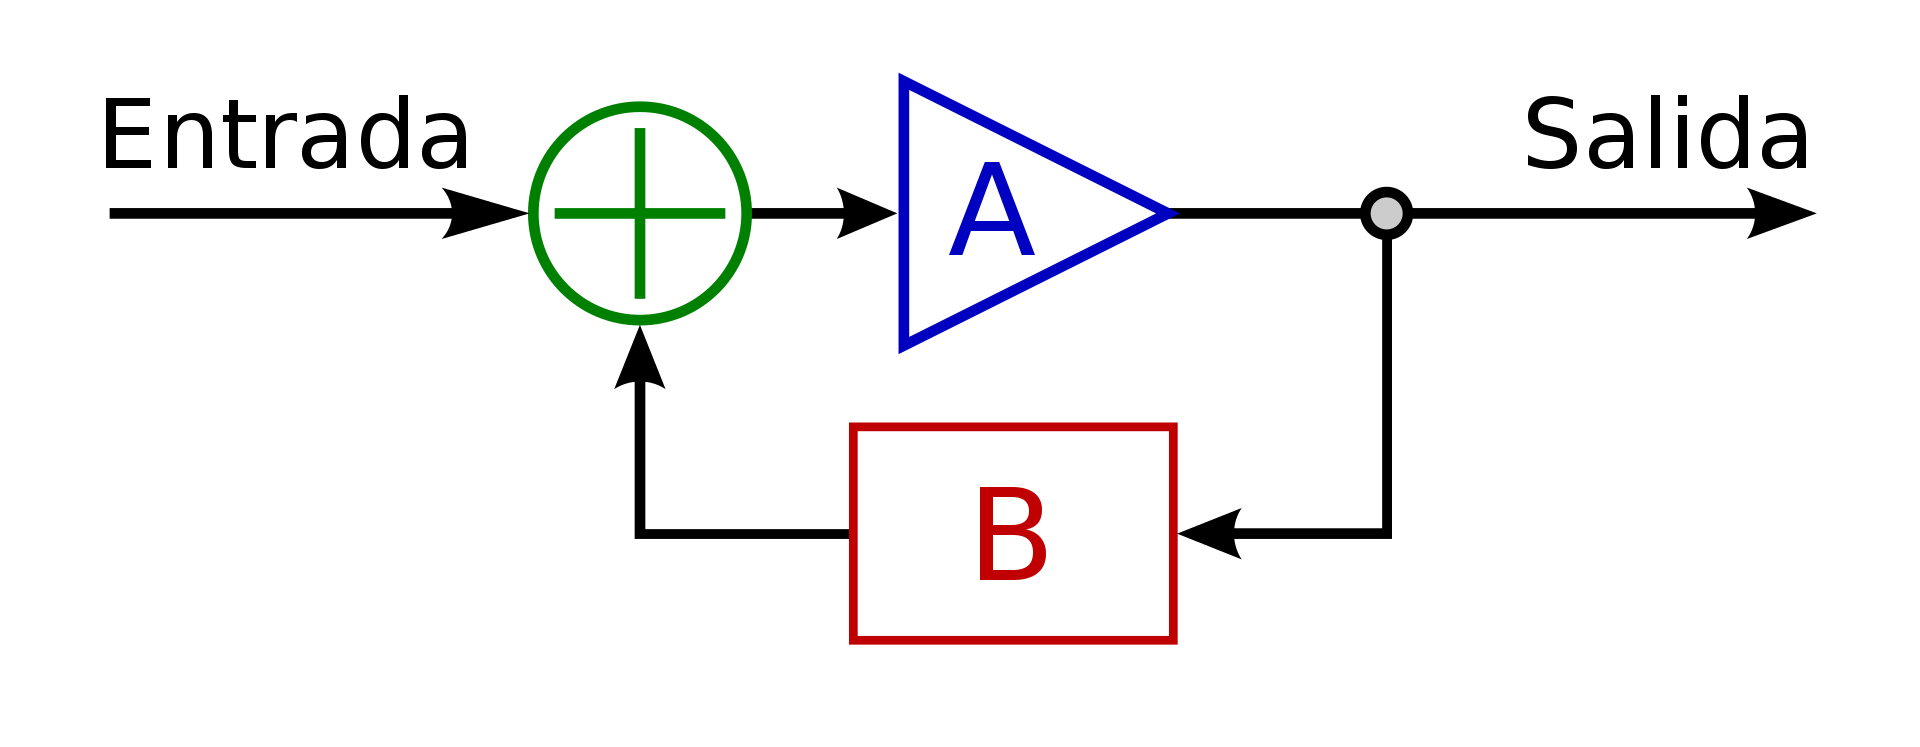
\includegraphics[width=8cm]{Imagenes/1.png}
            \caption{Estructura básica de un oscilador con entrada igual a cero}
            \label{fig:1}
        \end{figure}
        
        Es la conexión entre la salida y la entrada de un oscilador que permite mantener y regenerar la señal oscilante. Proporciona la realimentación positiva necesaria para que el oscilador genere señales de forma autónoma y continua. La estructura básica de un oscilador sinodal consta de un amplificador en un lazo de realimentación positiva, como se muestra en el diagrama de bloques de la figura \ref{fig:1}. Es importante observar que, a diferencia del lazo de realimentación negativa, aquí la señal de realimentación \(x_f\) se suma con un signo positivo. Entonces, la ganancia de realimentación está dada por


        \begin{equation}
            A(s) = \frac{A(s)}{1 - A(s)\beta(s)} \label{eqn:7}
        \end{equation}

        Donde se observa el signo negativo en el denominador
        La ganancia de lazo del circuito de la figura es \( -A(s)\beta(s) \), pero para nuestro propósito aquí, es más conveniente cancelar el signo menos y definir la ganancia de lazo \( L(s) \) como

        \begin{equation}
            L(s) = A(s)\beta(s)
        \end{equation}


        La ecuación característica se convierte entonces en

        \begin{equation}
            -L(s) + 1 = 0
        \end{equation}
        
    \subsection{Criterio de Barkhausen}

        Si a una frecuencia específica \(f_0\) la ganancia de lazo \(A\beta\) es igual a la unidad, se deduce de la ecuación (7) que \(Af\) será infinita. Esto es, a esta frecuencia, el circuito tendrá una salida finita para la señal de entrada cero. Este circuito es, por definición, un oscilador. Entonces, la condición para que el lazo de realimentación de la ilustración 2 produzca oscilaciones sinodales de frecuencia \(w_0\) es que
        
        \begin{equation}
            A(s)\beta(s) = 1
        \end{equation}

        En otras palabras, el criterio de Barkhausen establece las condiciones necesarias para que un oscilador genere señales de forma sostenida:

    \subsection{Oscilador básico de puente de Wien}
    

        \begin{figure}[H]
            \centering
            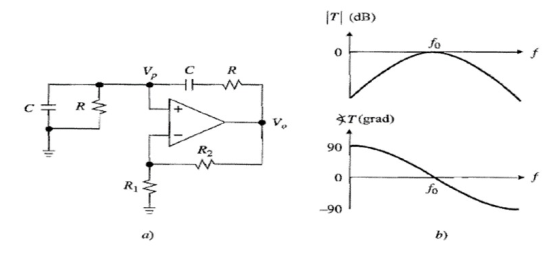
\includegraphics[width=10cm]{Imagenes/3.png}
            \caption{Puente de Wien con su Diagrama de Bode en amplitud y fase}
            \label{fig:3}
        \end{figure}
        
        Es un oscilador que utiliza un amplificador operacional realimentado con un puente resistivo-capacitivo para generar oscilaciones sinusoidales. La frecuencia de oscilación depende de los valores de \(R\) y \(C\) del puente.

    \subsection{Control de Amplitud}
        Son técnicas utilizadas en los osciladores para estabilizar y limitar la amplitud de oscilación. Por ejemplo, mediante diodos en el circuito resonante o control automático de ganancia en el amplificador.

        \begin{figure}[H]
            \centering
            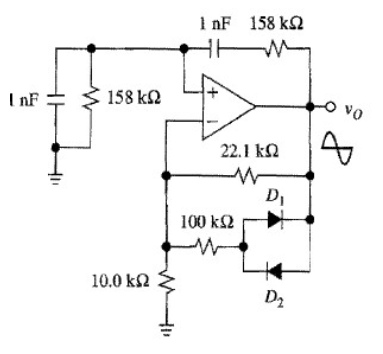
\includegraphics[width=8cm]{Imagenes/4.png}
            \caption{Oscildor con control de amplitud}
            \label{fig:4}
        \end{figure}

        El circuito de la figura \ref{fig:4} utiliza un circuito simple diodo-resistor para controlar el valor efectivo de R2. En niveles de señal bajos, los diodos están apagados, por lo tanto, la resistencia de \(100k\Omega\) no tiene ningún efecto. Entonces, se tiene que \(\frac{R2}{R1} = \frac{22.1}{10} = 2.21\), o bien \(T(jf_0) = \frac{(1 + 2.21)}{3} = 1.07 > 1\), lo que indica el surgimiento de la oscilación. Conforme la oscilación crece, los diodos son llevados de forma gradual a la conducción en medios ciclos alternados. En el límite de la conducción fuerte del diodo, efectivamente, \(R2\) cambiaría a \(18.1k\Omega\), donde se obtiene \(T(jf_0) = 0.937 < 1\). Sin embargo, antes de que alcance esta condición límite, la amplitud se estabilizará automáticamente en algún nivel intermedio de la conducción del diodo donde \(\frac{R2}{R1} = 2\) exactamente, o \(T(jf_0) = 1\).

        \subsection{Multivibradores}

            Son osciladores digitales que generan señales cuadradas o Rectangulares. Están formados por amplificadores realimentados con circuitos RC para controlar los tiempos de conmutación. Se clasifican en: Astable y monoestable.

            \subsubsection*{Multivibrador Astable}

                Multivibrador que no tiene estado estable, sino que conmuta continuamente entre
                dos estados. Genera una onda cuadrada periódica cuya frecuencia depende de los valores
                de \(R\) y \(C\).
                
                \subsubsection*{Multivibrador Monoestable}
                
                Multivibrador que tiene un estado estable y uno inestable. Al recibir un pulso de
                disparo cambia al estado inestable durante un tiempo determinado para luego volver al
                estado estable. Genera un único pulso rectangular por cada pulso de disparo.

            \subsection*{Generador de Funciones}

                Circuito electrónico capaz de generar diferentes formas de onda programables
                (senoidal, triangular, cuadrada, rampa, etc). Suele basarse en un oscilador controlado por
                voltaje (VCO).
                
                \subsection*{Histéresis}
                
                Es el fenómeno por el cual el estado de salida de un sistema depende de su estado
                anterior. Se utiliza en comparadores para evitar conmutaciones erráticas debido al ruido.
                
                \subsection*{Comparador}
                
                Circuito que compara dos señales de entrada y produce una salida determinada
                por la relación entre ellas. Tiene dos niveles de salida posibles, alto y bajo. Se usa en
                sistemas de instrumentación, convertidores A/D, etc.
                
                \subsection*{Comparador por Histéresis}
                
                Comparador diseñado intencionalmente para exhibir histéresis, los comparadores
                también pueden ser realimentados, solo que en su caso resulta más beneficiosa la
                realimentación positiva en la zona lineal, que la negativa comúnmente usada en los
                amplificadores operacionales. Al practicar la realimentación positiva en un comparador
                se obtiene fundamentalmente un nuevo comportamiento conocido como histéresis, en el
                cual los niveles de conmutación cambian con el estado (nivel de tensión) que se encuentre
                en dicho circuito.
                
                \subsection*{Generador de Onda Triangular}
                
                Circuito que genera una señal triangular, alternando rampas de subida y bajada. Se
                implementa cargando/descargando un capacitor entre dos niveles de voltaje con una
                constante de tiempo fija.




               

\newpage
